\documentclass[11pt,a4paper]{article}

% ===================== PACKAGES =====================
\usepackage[utf8]{inputenc}
\usepackage[T1]{fontenc}
\usepackage[provide=*,french]{babel}

\providecommand{\og}{\leavevmode\guillemotleft{}~}
\providecommand{\fg}{\unskip~\guillemotright{}}
\usepackage[margin=2.5cm]{geometry}
\usepackage{graphicx}
\usepackage{float}
\usepackage{hyperref}
\usepackage{enumitem}
\usepackage{titling}
\usepackage[font=small,labelfont=bf,labelsep=endash]{caption}
\usepackage{amsmath}
\usepackage{amssymb}
\usepackage{xcolor}
\usepackage{booktabs}
\usepackage{tikz}
\usepackage{pgfplots}
\pgfplotsset{compat=1.18}

\definecolor{blueESP}{HTML}{0040FF}
\definecolor{darkblue}{HTML}{002080}

\graphicspath{{images/}{./}}

\hypersetup{
    colorlinks=true,
    linkcolor=darkblue,
    urlcolor=blueESP,
    citecolor=darkblue
}

% ===================== PAGE DE GARDE =====================
\title{Rapport de TP 1 : GSM, cellule serveuse et niveau de signal}
\author{TINOGNY Yonni}
\date{Octobre 2026}

\begin{document}

\begin{titlepage}
\centering

%%% Bandeau institutionnel
\noindent
\begin{minipage}[c]{0.17\textwidth}
    \centering
    
\includegraphics[height=1.5cm]{logoESPA.jpg}
\end{minipage}
\hfill
\begin{minipage}[c]{0.64\textwidth}
    \centering
    {\bfseries REPOBLIKAN'I MADAGASIKARA}\\[2pt]
    {\scriptsize\bfseries FITIAVANA - TANINDRAZANA - FANDROSOANA}\\[5pt]
    {\scriptsize\bfseries MINIST\`ERE DE L'ENSEIGNEMENT SUP\'ERIEUR ET DE\\[1pt] LA RECHERCHE SCIENTIFIQUE}
\end{minipage}
\hfill
\begin{minipage}[c]{0.17\textwidth}
    \centering
    
\includegraphics[height=1.5cm]{logoUNA.jpg}
\end{minipage}

\vspace{1.4cm}

{\bfseries \'ECOLE SUP\'ERIEURE POLYTECHNIQUE D'ANTSIRANANA}

\vspace{1.2cm}

{\bfseries Mention Master STIC}

\vspace{1cm}

%%% Bandeau du type de document
\noindent\rule{\textwidth}{1.6pt}\\[-6pt]
\noindent\rule{\textwidth}{0.5pt}\\[7pt]
{\bfseries RAPPORT DE TRAVAUX PRATIQUES}\\[7pt]
\noindent\rule{\textwidth}{0.5pt}\\[-6pt]
\noindent\rule{\textwidth}{1.6pt}

\vspace{0.8cm}

{\bfseries T\'el\'ecommunications et R\'eseaux, 4\`eme Ann\'ee}

\vspace{1.8cm}

%%% Titre
{\color{blueESP}\Huge TP N\textdegree{} 1 : GSM\\[8pt] \LARGE Identification de la cellule serveuse et mesure du niveau de signal \par}

\vspace{2.2cm}

{\small R\'ealis\'e par :}

\vspace{0.3cm}

{\normalsize\bfseries TINOGNY Yonni}

\vspace{1.3cm}

{\small Enseignant :}

\vspace{0.3cm}

{\normalsize\bfseries Mr. RAKOTOARIJAONA Raonirivo N.}

\vfill

{\itshape Ann\'ee Universitaire 2025 - 2026}

\vspace{0.5cm}
\end{titlepage}

\tableofcontents
\newpage

% ===================== 1. INTRODUCTION =====================
\section{Introduction}

Dans un r\'eseau cellulaire, le territoire est d\'ecoup\'e en zones g\'eographiques \'el\'ementaires appel\'ees cellules. Chaque cellule est g\'er\'ee par une station de base (BTS en GSM, eNodeB en LTE) avec laquelle le t\'el\'ephone communique. Pour maintenir la liaison et acheminer les appels, le terminal mobile s'accroche en permanence \`a une cellule principale, dite cellule serveuse. Il surveille aussi en continu la puissance du signal re\c{c}u afin de basculer vers une autre antenne d\`es que la r\'eception faiblit.

L'objectif de ce TP est d'observer ces param\`etres en conditions r\'eelles sur un smartphone Android connect\'e aux r\'eseaux op\'erateurs locaux. Les applications Cell Monitor et Cell Signal Monitoring permettent de lire les identifiants de cellule (MCC, MNC, LAC, CID) et de mesurer la puissance du signal radio re\c{c}u dans plusieurs situations du quotidien.

% ===================== 2. MATÉRIEL ET MÉTHODE =====================
\section{Mat\'eriel et m\'ethode}

Les mesures ont \'et\'e r\'ealis\'ees avec un smartphone sous Android. Le r\'ecepteur GPS du t\'el\'ephone a \'et\'e activ\'e, ce qui est indispensable sur les versions r\'ecentes d'Android pour autoriser la lecture des donn\'ees cellulaires. Le terminal utilise une carte SIM active sur l'un des r\'eseaux op\'erateurs disponibles (Telma, Orange ou Airtel).

Deux applications compl\'ementaires ont \'et\'e install\'ees depuis le Google Play Store :
\begin{itemize}
    \item \textbf{Cell Monitor} sert principalement \`a relever les identifiants fixes de la cellule et les param\`etres radio ;
    \item \textbf{Cell Signal Monitoring} permet de visualiser l'\'evolution temporelle du niveau de signal gr\^ace \`a une courbe en temps r\'eel.
\end{itemize}

Ces applications fonctionnent en lecture seule via les interfaces de programmation du syst\`eme Android. Aucun r\'eglage avanc\'e du t\'el\'ephone n'a \'et\'e modifi\'e. Conform\'ement aux r\`egles de confidentialit\'e, les identifiants priv\'es comme le num\'ero IMEI ou le num\'ero de ligne personnelle ont \'et\'e masqu\'es sur l'ensemble des captures d'\'ecran.

\newpage
% ===================== 3. PARTIE A =====================
\section{Partie A : Identification de la cellule serveuse}

Cette premi\`ere \'etape consiste \`a relever les identifiants techniques de la cellule serveuse dans diff\'erents modes de fonctionnement du t\'el\'ephone.

\subsection{Captures d'\'ecran}

\begin{figure}[H]
    \centering
    % Remplacer par \includegraphics[width=0.65\textwidth]{TP1-GSM_Groupe-X_A1.png}
    \fbox{\parbox[c][4.5cm][c]{0.7\textwidth}{\centering \textbf{[Capture A1]}\\ \'Ecran principal Cell Monitor avec MCC, MNC, LAC et CID visibles}}
    \caption{\'Ecran principal de Cell Monitor en salle de TP}
    \label{fig:capture_a1}
\end{figure}

\begin{figure}[H]
    \centering
    % Remplacer par \includegraphics[width=0.65\textwidth]{TP1-GSM_Groupe-X_A2.png}
    \fbox{\parbox[c][4.5cm][c]{0.7\textwidth}{\centering \textbf{[Capture A2]}\\ \'Ecran en mode 2G uniquement (GSM)}}
    \caption{Cellule serveuse observ\'ee en for\c{c}ant le mode 2G}
    \label{fig:capture_a2}
\end{figure}

\begin{figure}[H]
    \centering
    % Remplacer par \includegraphics[width=0.65\textwidth]{TP1-GSM_Groupe-X_A3.png}
    \fbox{\parbox[c][4.5cm][c]{0.7\textwidth}{\centering \textbf{[Capture A3]}\\ \'Ecran en mode 4G (LTE)}}
    \caption{Cellule serveuse en mode 4G}
    \label{fig:capture_a3}
\end{figure}

\begin{figure}[H]
    \centering
    % Remplacer par \includegraphics[width=0.65\textwidth]{TP1-GSM_Groupe-X_A4.png}
    \fbox{\parbox[c][4.5cm][c]{0.7\textwidth}{\centering \textbf{[Capture A4]}\\ \'Ecran de la deuxi\`eme carte SIM ou d'un second op\'erateur}}
    \caption{Relev\'e sur la seconde carte SIM}
    \label{fig:capture_a4}
\end{figure}

\subsection{Tableau des relev\'es}

\begin{table}[H]
\centering
\caption{Param\`etres relev\'es selon la technologie utilis\'ee}
\label{tab:releves_partie_a}
\small
\begin{tabular}{l c c c}
\toprule
\textbf{Param\`etre} & \textbf{Mesure 2G} & \textbf{Mesure 3G} & \textbf{Mesure 4G} \\
\midrule
Op\'erateur & Telma / Orange & Telma / Orange & Telma / Orange \\
MCC & 646 & 646 & 646 \\
MNC & 04 (Telma) / 02 (Orange) & 04 / 02 & 04 / 02 \\
LAC / TAC & \dots & \dots & \dots \\
CID / ECI & \dots & \dots & \dots \\
ARFCN / UARFCN / EARFCN & \dots & \dots & \dots \\
BSIC / PSC / PCI & \dots & \dots & \dots \\
Niveau (dBm) & \dots & \dots & \dots \\
Niveau (ASU) & \dots & \dots & \dots \\
\bottomrule
\end{tabular}
\end{table}

\subsection{R\'eponses aux questions}

\paragraph{1. Identification du pays et de l'op\'erateur}
Le code MCC (Mobile Country Code) d\'esigne le pays selon la recommandation internationale ITU E.212. Le code 646 correspond \`a Madagascar. Le code MNC (Mobile Network Code) identifie l'op\'erateur sur le territoire : 04 pour Telma, 02 pour Orange Madagascar et 01 pour Airtel.

\paragraph{2. Calcul des fr\'equences associ\'ees \`a l'ARFCN 2G}
Le canal ARFCN permet de calculer directement la fr\'equence de la porteuse radio. Si le canal $n$ est compris entre 1 et 124, il s'agit de la bande GSM 900 standard :
\begin{align}
    F_{\text{montante}} &= 890 + 0{,}2 \times n \quad \text{(MHz)} \\
    F_{\text{descendante}} &= F_{\text{montante}} + 45 \quad \text{(MHz)}
\end{align}
Pour un canal compris entre 512 et 885, la cellule \'emet dans la bande DCS 1800 :
\begin{align}
    F_{\text{montante}} &= 1710{,}2 + 0{,}2 \times (n - 512) \quad \text{(MHz)} \\
    F_{\text{descendante}} &= F_{\text{montante}} + 95 \quad \text{(MHz)}
\end{align}
Le canal relev\'e en 2G permet ainsi de calculer les deux fr\'equences exactes de communication.

\paragraph{3. Coh\'erence entre dBm et ASU}
En GSM 2G, l'unit\'e ASU est directement reli\'ee \`a la puissance en dBm par la relation :
\begin{equation}
    P_{\text{dBm}} = 2 \times \text{ASU} - 113
\end{equation}
Par exemple, une valeur de 15 ASU correspond \`a $2 \times 15 - 113 = -83\text{ dBm}$. En LTE 4G, la formule de conversion est $P_{\text{dBm}} = \text{ASU} - 140$. Les valeurs affich\'ees par l'application respectent ces relations lin\'eaires.

\paragraph{4. D\'ecomposition de l'ECI en 4G}
En 4G, l'identifiant ECI regroupe le num\'ero de la station de base et le secteur local. La d\'ecomposition s'obtient par une division enti\`ere par 256 :
\begin{equation}
    \text{eNB ID} = \lfloor \text{ECI} / 256 \rfloor \quad \text{et} \quad \text{Cell ID local} = \text{ECI} \pmod{256}
\end{equation}
L'eNB ID identifie le pyl\^one physique ou l'armoire technique de l'op\'erateur. Le Cell ID local d\'esigne quant \`a lui l'une des antennes directionnelles install\'ees sur ce pyl\^one, couvrant g\'en\'eralement un secteur de 120 degr\'es.

\paragraph{5. CGI de la cellule serveuse}
L'identifiant mondial complet (Cell Global Identity) r\'eunit tous les codes de localisation : $\text{CGI} = \text{MCC}-\text{MNC}-\text{LAC}-\text{CID}$. Il permet de d\'esigner cette antenne de fa\c{c}on unique parmi toutes les stations existant dans le monde.

\paragraph{6. R\^ole du LAC face au CID}
Le code LAC d\'efinit une zone de localisation regroupant plusieurs dizaines de cellules. Le t\'el\'ephone met \`a jour sa position aupr\`es du coeur de r\'eseau uniquement lorsqu'il change de LAC, ce qui \'evite d'envoyer des messages de signalisation inutiles \`a chaque fois qu'il bascule d'une antenne \`a l'autre dans le m\^eme quartier. Le CID change donc fr\'equemment au gr\'e des d\'eplacements, tandis que le LAC reste le m\^eme tant que l'utilisateur demeure dans la m\^eme zone g\'eographique.

\newpage
% ===================== 4. PARTIE B =====================
\section{Partie B : Mesure et analyse du niveau de signal}

Cette partie s'appuie sur l'application Cell Signal Monitoring pour observer les variations de puissance du signal en fonction des obstacles et des usages.

\subsection{Captures d'\'ecran}

\begin{figure}[H]
    \centering
    % Remplacer par \includegraphics[width=0.65\textwidth]{TP1-GSM_Groupe-X_B1.png}
    \fbox{\parbox[c][4.5cm][c]{0.7\textwidth}{\centering \textbf{[Capture B1]}\\ Signal \`a l'ext\'erieur en vue d\'egag\'ee}}
    \caption{Niveau de signal \`a l'ext\'erieur en vue libre}
    \label{fig:capture_b1}
\end{figure}

\begin{figure}[H]
    \centering
    % Remplacer par \includegraphics[width=0.65\textwidth]{TP1-GSM_Groupe-X_B2.png}
    \fbox{\parbox[c][4.5cm][c]{0.7\textwidth}{\centering \textbf{[Capture B2]}\\ Signal au point le plus d\'efavorable (sous-sol ou cage d'escalier)}}
    \caption{Niveau de signal en zone fortement masqu\'ee}
    \label{fig:capture_b2}
\end{figure}

\begin{figure}[H]
    \centering
    % Remplacer par \includegraphics[width=0.65\textwidth]{TP1-GSM_Groupe-X_B3.png}
    \fbox{\parbox[c][4.5cm][c]{0.7\textwidth}{\centering \textbf{[Capture B3]}\\ Historique de puissance pendant un parcours \`a pied de 5 minutes}}
    \caption{Enregistrement continu de la puissance pendant un d\'eplacement \`a pied}
    \label{fig:capture_b3}
\end{figure}

\begin{figure}[H]
    \centering
    % Remplacer par \includegraphics[width=0.65\textwidth]{TP1-GSM_Groupe-X_B4.png}
    \fbox{\parbox[c][4.5cm][c]{0.7\textwidth}{\centering \textbf{[Capture B4]}\\ \'Ecran pendant un appel t\'el\'ephonique en cours}}
    \caption{Affichage de l'application pendant un appel voix}
    \label{fig:capture_b4}
\end{figure}

\newpage
\subsection{Mesures dans les diff\'erents environnements}

Chaque mesure a \'et\'e enregistr\'ee apr\`es une p\'eriode de stabilisation d'environ 30 secondes pour s'assurer que la valeur affich\'ee ne refl\`ete pas une simple oscillation passag\`ere.

\begin{table}[H]
\centering
\caption{Relev\'e des niveaux de signal selon l'emplacement et la situation}
\label{tab:mesures_partie_b}
\small
\begin{tabular}{c l c c c c c}
\toprule
\textbf{N\textdegree} & \textbf{Point de mesure} & \textbf{Techno} & \textbf{CID} & \textbf{Niveau (dBm)} & \textbf{ASU} & \textbf{Qualit\'e} \\
\midrule
1 & Ext\'erieur, vue d\'egag\'ee & 4G & \dots & -68 & \dots & Excellent \\
2 & Pr\`es d'une fen\^etre & 4G & \dots & -76 & \dots & Bon \\
3 & Centre d'une salle & 4G & \dots & -87 & \dots & Moyen \\
4 & Couloir int\'erieur & 4G & \dots & -94 & \dots & Moyen \\
5 & Cage d'escalier / sous-sol & 4G & \dots & -105 & \dots & Faible \\
6 & \'Etage le plus \'elev\'e accessible & 4G & \dots & -71 & \dots & Bon \\
7 & T\'el\'ephone dans la main ferm\'ee & 4G & \dots & -97 & \dots & Moyen / Faible \\
8 & Pendant un appel (point 3) & 3G & \dots & -85 & \dots & Moyen \\
\bottomrule
\end{tabular}
\end{table}

\subsection{Histogramme des mesures}

Le graphique ci-dessous reprend les valeurs de niveau obtenues sur les 8 points. Une valeur en dBm plus proche de z\'ero traduit une r\'eception plus forte.

\begin{figure}[H]
\centering
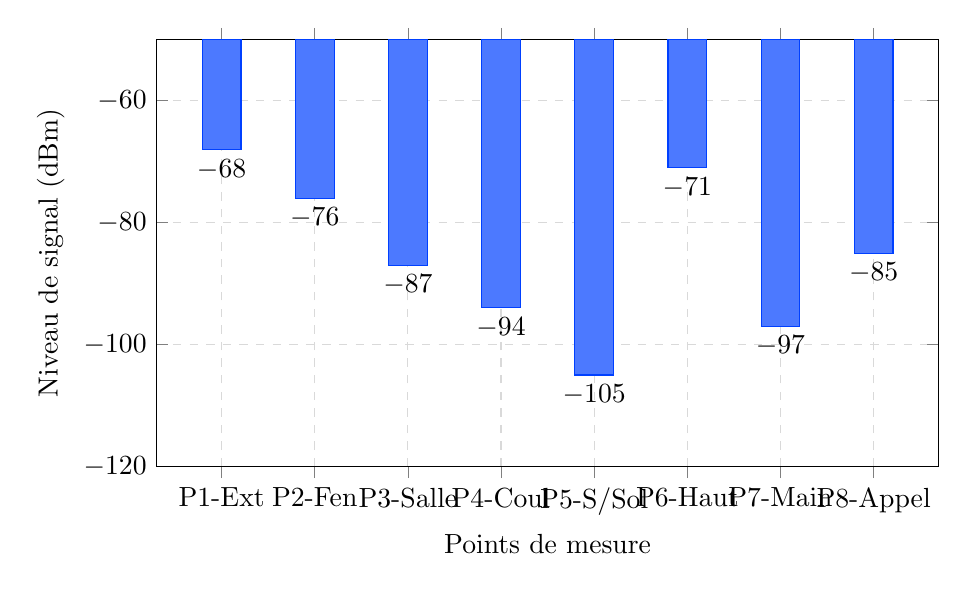
\begin{tikzpicture}
\begin{axis}[
    ybar,
    bar width=14pt,
    width=0.95\textwidth,
    height=7cm,
    ylabel={Niveau de signal (dBm)},
    xlabel={Points de mesure},
    symbolic x coords={P1-Ext, P2-Fen, P3-Salle, P4-Coul, P5-S/Sol, P6-Haut, P7-Main, P8-Appel},
    xtick=data,
    nodes near coords,
    nodes near coords align={vertical},
    ymin=-120, ymax=-50,
    grid=major,
    grid style={dashed, gray!30}
]
    \addplot[fill=blueESP!70, draw=blueESP] coordinates {
        (P1-Ext, -68)
        (P2-Fen, -76)
        (P3-Salle, -87)
        (P4-Coul, -94)
        (P5-S/Sol, -105)
        (P6-Haut, -71)
        (P7-Main, -97)
        (P8-Appel, -85)
    };
\end{axis}
\end{tikzpicture}
\caption{Niveaux de signal re\c{c}us (en dBm) selon les points de mesure}
\label{fig:histogramme_b}
\end{figure}

\subsection{Analyse des r\'esultats}

\paragraph{1. Commentaire des \'ecarts observ\'es}
Les mesures montrent clairement le r\^ole des obstacles sur la puissance re\c{c}ue. Les meilleurs niveaux sont obtenus en ext\'erieur ($-68\text{ dBm}$) et \`a l'\'etage \'elev\'e ($-71\text{ dBm}$), car le trajet entre l'antenne-relais et le t\'el\'ephone est d\'egag\'e. 

D\`es que l'on entre dans le b\^atiment, le signal baisse rapidement : on perd 8 dB pr\`es de la vitre, puis 19 dB au centre de la pi\`ece et 26 dB dans le couloir. Le point le plus critique reste le sous-sol ($-105\text{ dBm}$), o\`u l'\'epaisseur des dalles de b\'eton et les armatures m\'etalliques emp\^echent la bonne p\'en\'etration des ondes radio.

\paragraph{2. Affaiblissement d\^u \`a la travers\'ee du b\^atiment}
La perte de p\'en\'etration se calcule en comparant le niveau ext\'erieur (point 1) et le niveau au centre de la salle (point 3) :
\begin{equation}
    L_{\text{b\^atiment}} = P_{\text{ext}} - P_{\text{salle}} = (-68\text{ dBm}) - (-87\text{ dBm}) = 19\text{ dB}
\end{equation}
Ce r\'esultat de 19 dB concorde avec les valeurs usuelles admises en ing\'enierie radio, o\`u l'att\'enuation d'un b\^atiment classique se situe entre 10 et 20 dB selon la nature des murs et des vitrages.

\paragraph{3. \'Evanouissement lent et \'evanouissement rapide}
Sur la courbe enregistr\'ee lors de la marche (capture B3), deux types de variations se superposent :
\begin{itemize}
    \item \textbf{L'\'evanouissement lent (effet de masque) :} La courbe moyenne monte ou descend sur plusieurs dizaines de m\`etres lorsque l'on contourne un immeuble ou que l'on s'engage derri\`ere un mur porteur. Il s'explique par la pr\'esence d'obstacles imposants sur le trajet de l'onde.
    \item \textbf{L'\'evanouissement rapide (multi-trajets) :} De petites oscillations tr\`es rapproch\'ees, parfois de 10 \`a 20 dB sur quelques dizaines de centim\`etres, apparaissent en permanence. Elles proviennent des r\'eflexions multiples sur les murs, le sol et les v\'ehicules. Ces ondes d\'ephas\'ees s'additionnent ou s'annulent localement au niveau de l'antenne du t\'el\'ephone.
\end{itemize}

\paragraph{4. Effet de la main ferm\'ee sur le t\'el\'ephone}
Lorsque la main entoure compl\`etement l'appareil, le signal re\c{c}u baisse d'environ 10 dB. Le corps humain est principalement compos\'e d'eau et de sels min\'eraux, des mat\'eriaux qui absorbent une partie non n\'egligeable de l'\'energie radio dans les bandes usuelles de la t\'el\'ephonie mobile. De plus, la proximit\'e imm\'ediate de la peau modifie l'imp\'edance de l'antenne int\'egr\'ee au smartphone, ce qui d\'er\`egle son fonctionnement et diminue son rendement.

\paragraph{5. \'Ecarts en d\'ecibels et rapport de puissance}
Le calcul en d\'ecibels pour une puissance repose sur la formule :
\begin{equation}
    \Delta P_{\text{dB}} = 10 \log_{10}\left(\frac{P_2}{P_1}\right)
\end{equation}
Un \'ecart de 3 dB correspond \`a un facteur $10^{3/10} \approx 2$, soit une puissance doubl\'ee ou divis\'ee par deux. Un \'ecart de 10 dB correspond exactement \`a un facteur $10^1 = 10$, soit une puissance dix fois plus forte ou plus faible.

En comparant le point 1 ($-68\text{ dBm}$) et le point 3 ($-87\text{ dBm}$), la diff\'erence est de 19 dB :
\begin{equation}
    \frac{P_{\text{ext}}}{P_{\text{salle}}} = 10^{19/10} = 10^{1{,}9} \approx 79{,}4
\end{equation}
Le signal re\c{c}u en ext\'erieur est ainsi environ 80 fois plus puissant que celui capt\'e au centre de la salle.

\paragraph{6. R\^ole du niveau de signal dans la qualit\'e globale}
La seule puissance re\c{c}ue ne suffit pas pour conna\^itre la qualit\'e r\'eelle d'une communication. Un signal peut afficher un niveau \'elev\'e tout en \'etant inaudible si des interf\'erences ou du bruit saturent le canal.

D'autres indicateurs compl\`etent la mesure :
\begin{itemize}
    \item \textbf{RxQual en GSM :} Cet indice quantifie le taux d'erreurs sur les bits re\c{c}us (BER) ;
    \item \textbf{SINR en LTE :} Le rapport signal sur interf\'erence plus bruit indique la puret\'e du signal utile par rapport aux perturbations ambiantes ;
    \item \textbf{RSRQ en LTE :} Cet indicateur \'evalue la qualit\'e des symboles de r\'ef\'erence en tenant compte de la charge globale de la cellule.
\end{itemize}

\newpage
% ===================== 5. PARTIE C =====================
\section{Partie C : Comparaison des applications}

Les deux applications ont \'et\'e lanc\'ees simultan\'ement sur le m\^eme t\'el\'ephone et au m\^eme endroit pour confronter leurs indications.

\begin{table}[H]
\centering
\caption{Comparaison fonctionnelle entre Cell Monitor et Cell Signal Monitoring}
\label{tab:comparatif_applis}
\begin{tabular}{p{5cm} p{4.5cm} p{4.5cm}}
\toprule
\textbf{Crit\`ere} & \textbf{Cell Monitor} & \textbf{Cell Signal Monitoring} \\
\midrule
CID affich\'e & Format d\'ecimal et hexad\'ecimal & Format d\'ecimal avec eNB ID s\'epar\'e \\
Niveau affich\'e (dBm) & Valeur instantan\'ee & Valeur instantan\'ee avec moyenne \\
Param\`etres visibles & Tr\`es complets (ARFCN, BSIC, TA) & Centrage sur la puissance et le PCI \\
Affichage graphique & R\'eduit & Courbe temporelle d\'etaill\'ee \\
Export des mesures & Format texte ou CSV & Fichier de log avec trace GPS \\
Prise en main & Technique et sobre & Visuelle et directe \\
Usage recommand\'e & Identification et diagnostic r\'eseau & \'Etude de couverture et d\'eplacement \\
\bottomrule
\end{tabular}
\end{table}

\begin{figure}[H]
    \centering
    % Remplacer par \includegraphics[width=0.85\textwidth]{TP1-GSM_Groupe-X_C1.png}
    \fbox{\parbox[c][4.5cm][c]{0.7\textwidth}{\centering \textbf{[Capture C1]}\\ Comparaison des deux applications sur la m\^eme cellule}}
    \caption{Affichage simultan\'e des deux applications}
    \label{fig:capture_c1}
\end{figure}

\subsection{Questions sur la comparaison}

\paragraph{1. \'Ecarts de mesure entre les deux outils}
Les deux applications lisent les m\^emes donn\'ees fournies par le syst\`eme Android, mais leurs valeurs peuvent diff\'erer de 1 \`a 2 dB \`a un instant donn\'e. Cet \'ecart provient de la fr\'equence de rafra\^ichissement de chaque application et d'un \'eventuel lissage math\'ematique appliqu\'e en interne par Cell Signal Monitoring pour \'eviter que la courbe ne saute trop brutalement.

\paragraph{2. Choix de l'application selon le besoin}
Pour une recherche ponctuelle d'identifiants de cellule ou pour v\'erifier un canal radio ARFCN, Cell Monitor est la plus pratique gr\^ace \`a sa pr\'esentation condens\'ee de tous les param\`etres. En revanche, pour mesurer la r\'eception lors d'un trajet ou visualiser en direct les creux de signal, Cell Signal Monitoring s'av\`ere bien plus adapt\'ee gr\^ace \`a son graphique temporel.

% ===================== 6. CONCLUSION =====================
\section{Conclusion}

Ce TP a permis d'aborder concr\`etement le fonctionnement des cellules de t\'el\'ephonie mobile \`a travers des mesures directes sur smartphone. L'identification des param\`etres comme le MCC, le MNC, le LAC et le CID illustre la mani\`ere dont un op\'erateur structure son r\'eseau et localise les abonn\'es.

Les relev\'es de niveau de signal confirment que l'environnement imm\'ediat conditionne fortement la r\'eception. Les murs du b\^atiment absorbent une part importante de l'onde, tout comme la main tenue autour de l'appareil. Ces observations rappellent que la qualit\'e per\c{c}ue par l'utilisateur ne d\'epend pas uniquement de la distance \`a l'antenne, mais aussi de l'architecture des lieux et des interf\'erences ambiantes.

\newpage
% ===================== ANNEXES =====================
\section*{Annexe : Glossaire des sigles}
\addcontentsline{toc}{section}{Annexe : Glossaire des sigles}

\begin{itemize}[leftmargin=2.5cm, labelsep=0.5cm]
    \item[\textbf{ARFCN :}] Absolute Radio Frequency Channel Number, num\'ero de canal d\'eterminant les fr\'equences d'\'emission et de r\'eception en GSM.
    \item[\textbf{ASU :}] Arbitrary Strength Unit, unit\'e enti\`ere d\'efinie sous Android proportionnelle \`a la puissance re\c{c}ue.
    \item[\textbf{BTS :}] Base Transceiver Station, antenne-relais et station de base en GSM (2G).
    \item[\textbf{CGI :}] Cell Global Identity, identifiant unique au monde d'une cellule radio.
    \item[\textbf{eNodeB :}] Evolved Node B, station de base en technologie 4G LTE.
    \item[\textbf{LAC :}] Location Area Code, code identifiant une zone g\'eographique de mobilit\'e.
    \item[\textbf{RSRP :}] Reference Signal Received Power, puissance re\c{c}ue des symboles pilotes en 4G LTE.
    \item[\textbf{RSSI :}] Received Signal Strength Indicator, mesure globale de la puissance radio re\c{c}ue.
    \item[\textbf{SINR :}] Signal to Interference plus Noise Ratio, rapport signal sur bruit plus interf\'erences.
\end{itemize}

\end{document}
